\section{Interface}

\subsection{Introduction}

Nous avons réalisé notre interface principalement sur base de nos usecases et overview diagrams ainsi que les choix effectués concernant la base de données et le class diagram.

\begin{flushleft}
Cette manière de procéder nous a permis de structurer nos idées afin de fournir l'interface la plus intuitive possible.
\end{flushleft}

\begin{flushleft}
De plus, nous avons décidé de séparer l'interface en \textbf{trois parties} :
\end{flushleft}

\begin{enumerate}[1.]
\item Le système de logs
\item L'interface client
\item L'interface fournisseur
\end{enumerate}

\begin{flushleft}
ce qui nous semblait plus approprié étant donné que nous devons obtenir deux applications distinctes, une pour le fournisseur et l'autre pour le client.
\end{flushleft}

\begin{flushleft}
Il est important de noter que nous avons utilisé le logiciel "Figma" pour réaliser ces maquettes.
\end{flushleft}

\newpage
\subsection{Système de logs}
Sur la page principale de connexion, l'utilisateur devra préciser s'il est client ou fournisseur en cochant la case apppropriée et pourra également changer de langue s'il le souhaite.
\begin{flushleft}
Il pourra dès lors entrer ses informations et \textbf{se connecter}.
\end{flushleft}

\begin{flushleft}
Cependant s'il a \textbf{oublié son mot de passe}, un bouton sera prévu à cet effet.
Ce dernier enverra l'utilisateur sur une nouvelle page où il devra inscrire le code qu'il aura reçu par mail et son nouveau mot de passe.
\end{flushleft}

\begin{flushleft}
Un bouton "Submit" aura pour but de confirmer ce que l'utilisateur a entré et un bouton "Back" sera présent si jamais ce dernier veut retourner en arrière.
\end{flushleft}


\begin{flushleft}
S'il n'a pas encore de compte, l'utilisateur aura la possibilité d'en \textbf{créer un nouveau}. 
Le sytème fonctionnera comme la connexion expliquée précédemment.
\end{flushleft}

\begin{flushleft}
La seule différence réside lorsque ce dernier appuiera sur le bouton "Create an account". 
L'utilisateur sera alors envoyé sur une nouvelle page où on lui demandera de confirmer la création de son compte en entrant le code qu'il aura reçu par mail pour plus de sécurité.
\end{flushleft}

\begin{flushleft}
Pour finir, de la même manière que pour le changement de mot de passe, un bouton "Finish" aura pour but de confirmer ce que l'utilisateur a entré et un bouton "Back" sera présent si jamais ce dernier veut retourner en arrière.
\end{flushleft}

\begin{flushleft}
En outre, l'utilisateur pourra demander qu'on lui renvoie un mail si le précédent n'est pas reçu.
\end{flushleft}\

\newpage
\begin{figure}
    \centering
    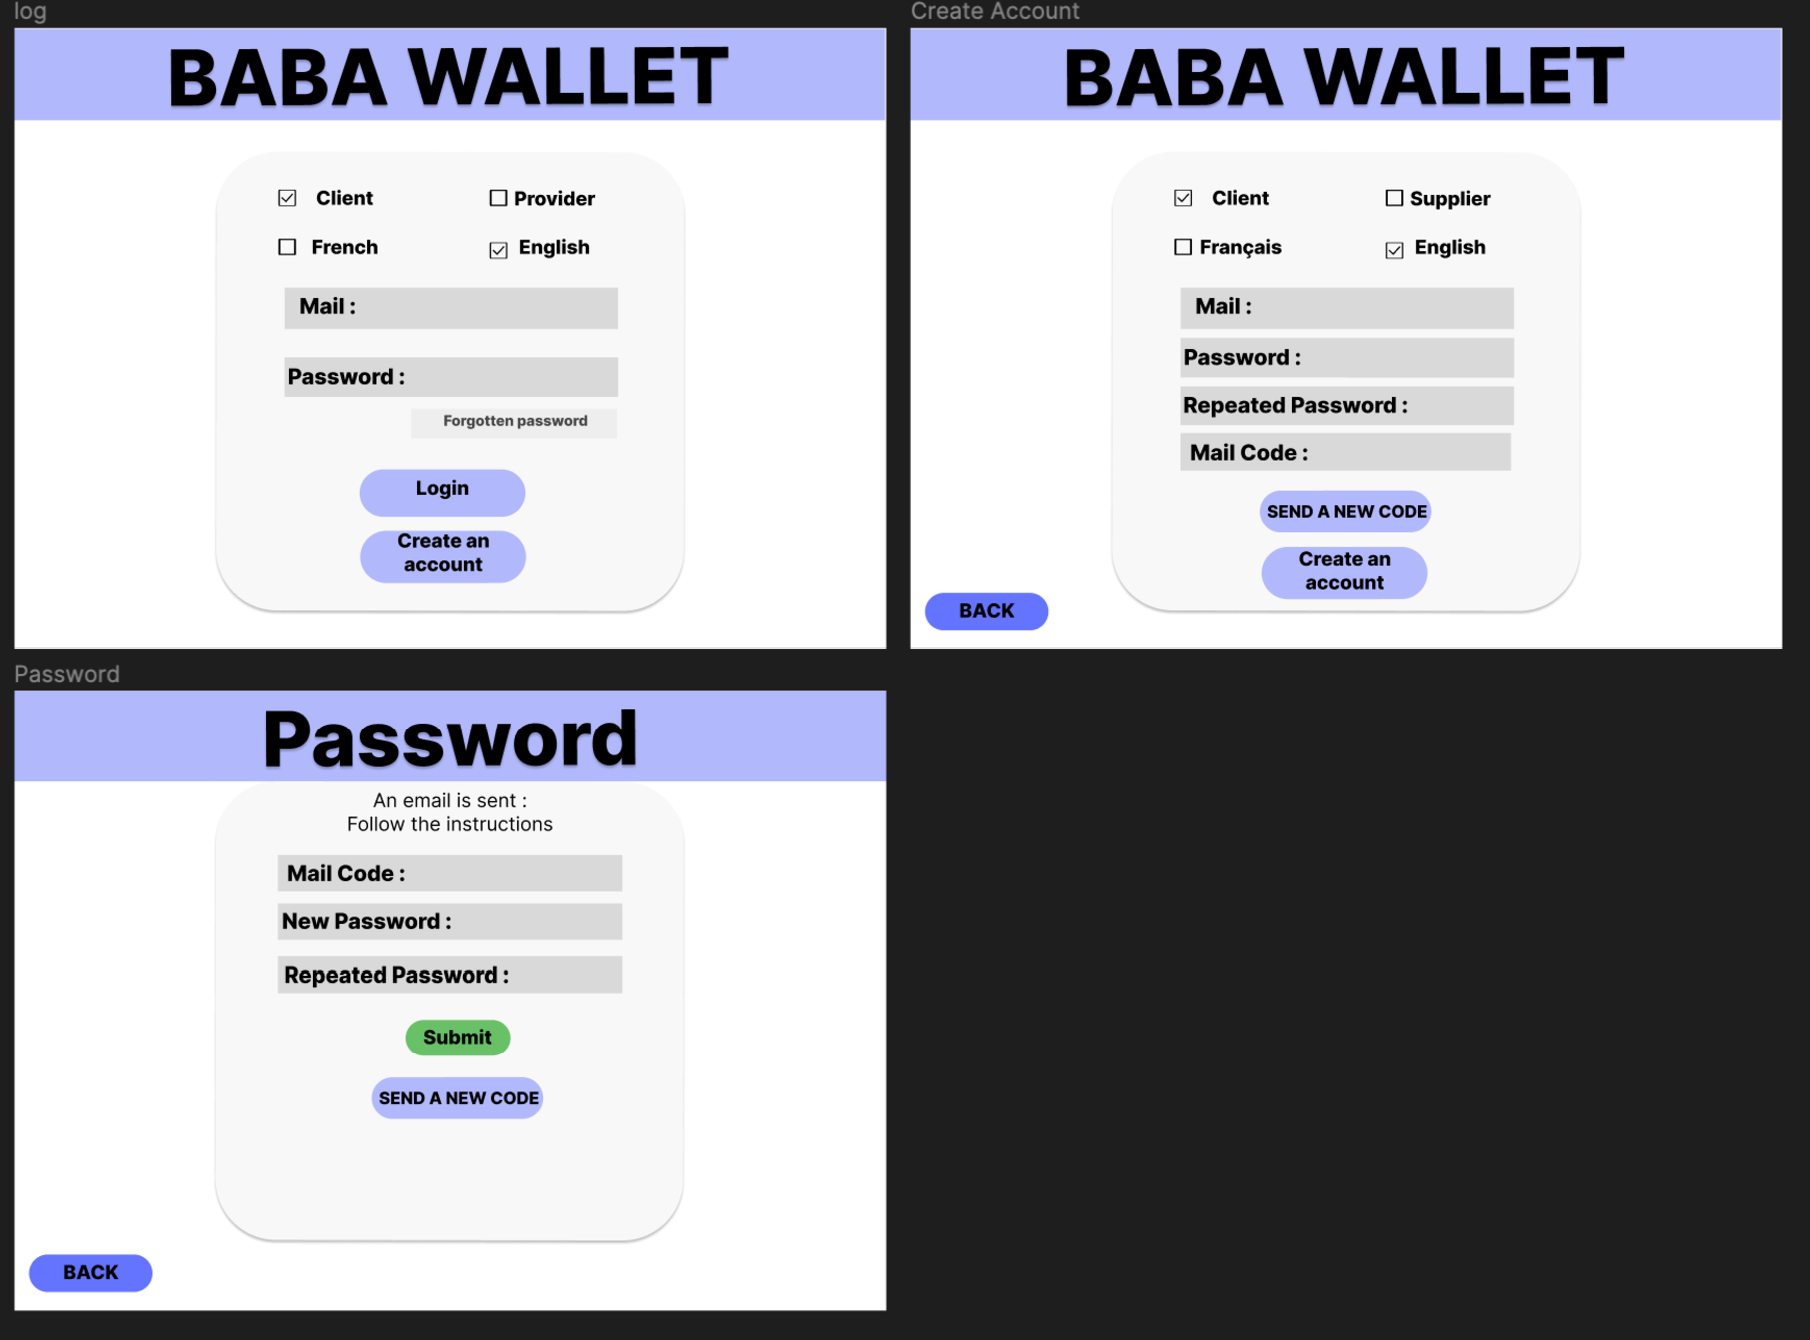
\includegraphics[width = 1\textwidth]{Base/interface/img/Log.pdf}
\end{figure}
\newpage
\subsection{Points communs}
Les points communs entre l'interface client et fournisseur sont
\begin{enumerate}
\item \textbf{Les notifications :}\newline
L'utilisateur verra le fournisseur ou client en question, le contexte et le contrat lié à la notification.\newline
Il pourra également observer plus en détail le contrat avec le bouton "See", marquer commme lue les notifications grâce au bouton "OK" et les accepter ou refuser dans le cadre d'une demande.\newline
En outre, la possibilité d'actualiser lui-même s'il le désire lui est laissée.
\item \textbf{Les paramètres :}\newline
Concernant le changement de mot de passe, cela se déroule exactement de la même manière que dans le système de logs.
Pour la langue, l'utilisateur pourra en ajouter, choisir sa préférée et changer celle étant active.\newline
Dans tous les cas, ce dernier sera conduit sur une page où il aura la possibilité de chercher une langue et ensuite soit de la télécharger, soit de la choisir en fonction du contexte.
\end{enumerate}



\newpage
\subsection{Interface client}

Lorsqu'un client se connectera, il arrivera sur la page d'acceuil ou plus précisément "Home".
\begin{flushleft}
Ce dernier aura alors les possibilités suivantes :
\end{flushleft}
\begin{enumerate}
\item Voir ses portefeuilles ("Wallets")
\item Voir ses contrats ("Your contracts")
\item Voir ses notifications
\item Voir les fournisseurs et contrats relatifs ("See new contracts")
\item Se déconnecter
\item Aller sur la page des paramètres
\end{enumerate}

\begin{flushleft}
Il est important de noter que ce n'est qu'à partir de ces six pages que le client pourra revenir sur la page "Home" étant donné le choix effectué dans notre overview diagram.
\end{flushleft}

\begin{flushleft}
Néanmoins, ce dernier aura la possibilité de revenir en arrière à l'aide du bouton "Back" lorsqu'il sera sur des "sous-pages" de ces six sections principales.
\end{flushleft}

\newpage
\begin{flushleft}
Nous pouvons maintenant commencer par l'option \textbf{"Voir ses portefeuilles" ("Wallets")} :
\end{flushleft}

\begin{flushleft}
Le client pourra à partir d'ici voir une liste reprenant tous les portefeuilles qu'il aura créé précédement. 
\end{flushleft}
\begin{flushleft}
Chaque rectangle représentant un portefeuille comprend :
\end{flushleft}
\begin{enumerate}
\item Le nom du portefeuille
\item Le nom du propriétaire du portefeuille
\item L'adresse associée au portefeuille
\end{enumerate}
\begin{flushleft}
Le bouton "Go" permettra de voir plus en détail un portefeuille et le bouton "+" sur le rectangle vide donnera la possibilité au client d'ajouter un nouveau portefeuille.
\end{flushleft}
\begin{flushleft}

Lorsqu'il souhaitera \textbf{voir plus en détail un portefeuille}, le client aura accès au nom du portefeuille, au nom du propriétaire du portefeuille et à l'adresse associée au porteuille comme sur la page précédente.
\end{flushleft}
\begin{flushleft}
Toutefois d'autres actions lui seront possibles :
\end{flushleft}
\begin{enumerate}
\item Voir ses dernières consommations
\item Voir les contrats associés
\item Voir les contrats associés en détail (Bouton "Go")
\item Ajouter des consommations (Bouton "Add consumptions")
\item Fermer définitivement le portefeuille (Bouton "Close the Wallet")
\end{enumerate}

\begin{flushleft}
Le bouton "Go" concernant les contrats associés l'amènera sur une page montrant le contrat que nous expliquerons prochainement.
\end{flushleft}

\begin{flushleft}
Le bouton \textbf{"Add consumptions"} l'entraînera vers une page où il pourra voir ses données de consommations en graphique ou en tableau à l'aide des deux boutons placés en haut de la page.
\end{flushleft}
\begin{flushleft}
Le réctangle gris les représentent et il pourra également séléctionner dans ce dernier s'il souhaite voir les données mensuellement, hebdomadairement,...
\end{flushleft}
\begin{flushleft}
Le client pourra également s'il le désire exporter ses données.
Nous pouvons noter que ce dernier exportera les données présentent dans le tableau gris au moment où il appuiera sur le bouton "Export".
\end{flushleft}
\begin{flushleft}
En ce qui concerne le changement et l'ajout de consommation, celui-ci devra entrer la date correspondante, le type d'énergie et la valeur associée et devra ensuite confirmer ses modifications grâce aux boutons "Change" et "Add".
\end{flushleft}

\begin{flushleft}
\textbf{Le bouton "+"} mentionné précédemment servant à ajouter un nouveau portefeuilles est connecté à une page qui lui demandera d'écrire le nom et l'adresse du nouveau portefeuille.
\end{flushleft}

\begin{flushleft}
Cette manière de procéder est liée au fait que nous avons décidé qu'un portefeuille doit être créé avant d'associer un contrat à ce dernier.
\end{flushleft}

\begin{flushleft}
La deuxième option est la suivante : \textbf{"Voir ses contrats" ("Your contracts")}
\end{flushleft}

\begin{flushleft}
Une fois sur cette page, le client aura accès à sa liste de contrats et il pourra rechercher un contrat spécifique en tapant le code "EAN" ou le nom du fournisseur.
\end{flushleft}

\begin{flushleft}
Les informations basiques qu'il verra sur chaque ligne de la liste sont le fournisseur et le type d'énergie.
\end{flushleft}

\begin{flushleft}
Lorsqu'il cliquera sur le \textbf{bouton "Go"} la nouvelle page lui offrira les informations suivantes : le type d'énergie et le fournisseur de la même manière que sur la page précédente.
\end{flushleft}
\begin{flushleft}
Les nouvelles informations disponibles sont les suivantes :
\end{flushleft}
\begin{enumerate}
\item Le nom du contrat
\item Le portefeuille associé (Le code "EAN" ainsi que l'adresse)
\item La localisation (du contrat)
\item Le prix basique
\item Le prix dépendant du jour et la nuit
\item Le taux fixe ou variable
\item Les heures creuses
\item La date d'ouverture du contrat
\item La date de fermeture du contrat
\end{enumerate}
\begin{flushleft}
Il pourra aussi fermer le contrat par le bouton "Close the contract".
\end{flushleft}

\newpage

\begin{flushleft}
La troisième et dernière section est \textbf{"Voir les fournisseurs et contrats relatifs ("See new contracts")"}
\end{flushleft}
\begin{flushleft}
Sur cette page, le client pourra voir une liste reprenant les noms des fournisseurs, les types d'énergies et la localisation pour chaque contrat.
\end{flushleft}
\begin{flushleft}
Pour lui rendre la tâche de recherche plus facile, nous avons mis à sa disposition une sélection sur le côté droit.
Cette dernière permettra de choisir le type d'énergie souhaité (Electricité, gaz et eau) ainsi que la localisation.
\end{flushleft}

\begin{flushleft}
Le \textbf{bouton "Go"} l'amènera sur les informations liées à un nouveau contrat :
\end{flushleft}
\begin{enumerate}
\item Le fournisseur
\item Le type d'énergie
\item La localisation (du contrat)
\item Le prix basique
\item Le prix dépendant du jour et la nuit
\item Le taux fixe ou variable
\item Les heures creuses
\item Le type de compteur
\end{enumerate}
\begin{flushleft}
Pour confirmer sa demande de contrat, le client devra entrer le nom du portefeuille auquel il souhaite l'associer ainsi que le code "EAN" et appuyer sur le bouton "Submit".
\end{flushleft}

\begin{flushleft}
Nous ne reviendrons pas sur les points "Voir les notifications" et "Les paramètres", ces derniers étant expliqués dans les points communs. 
\end{flushleft}

\begin{figure}
    \centering
    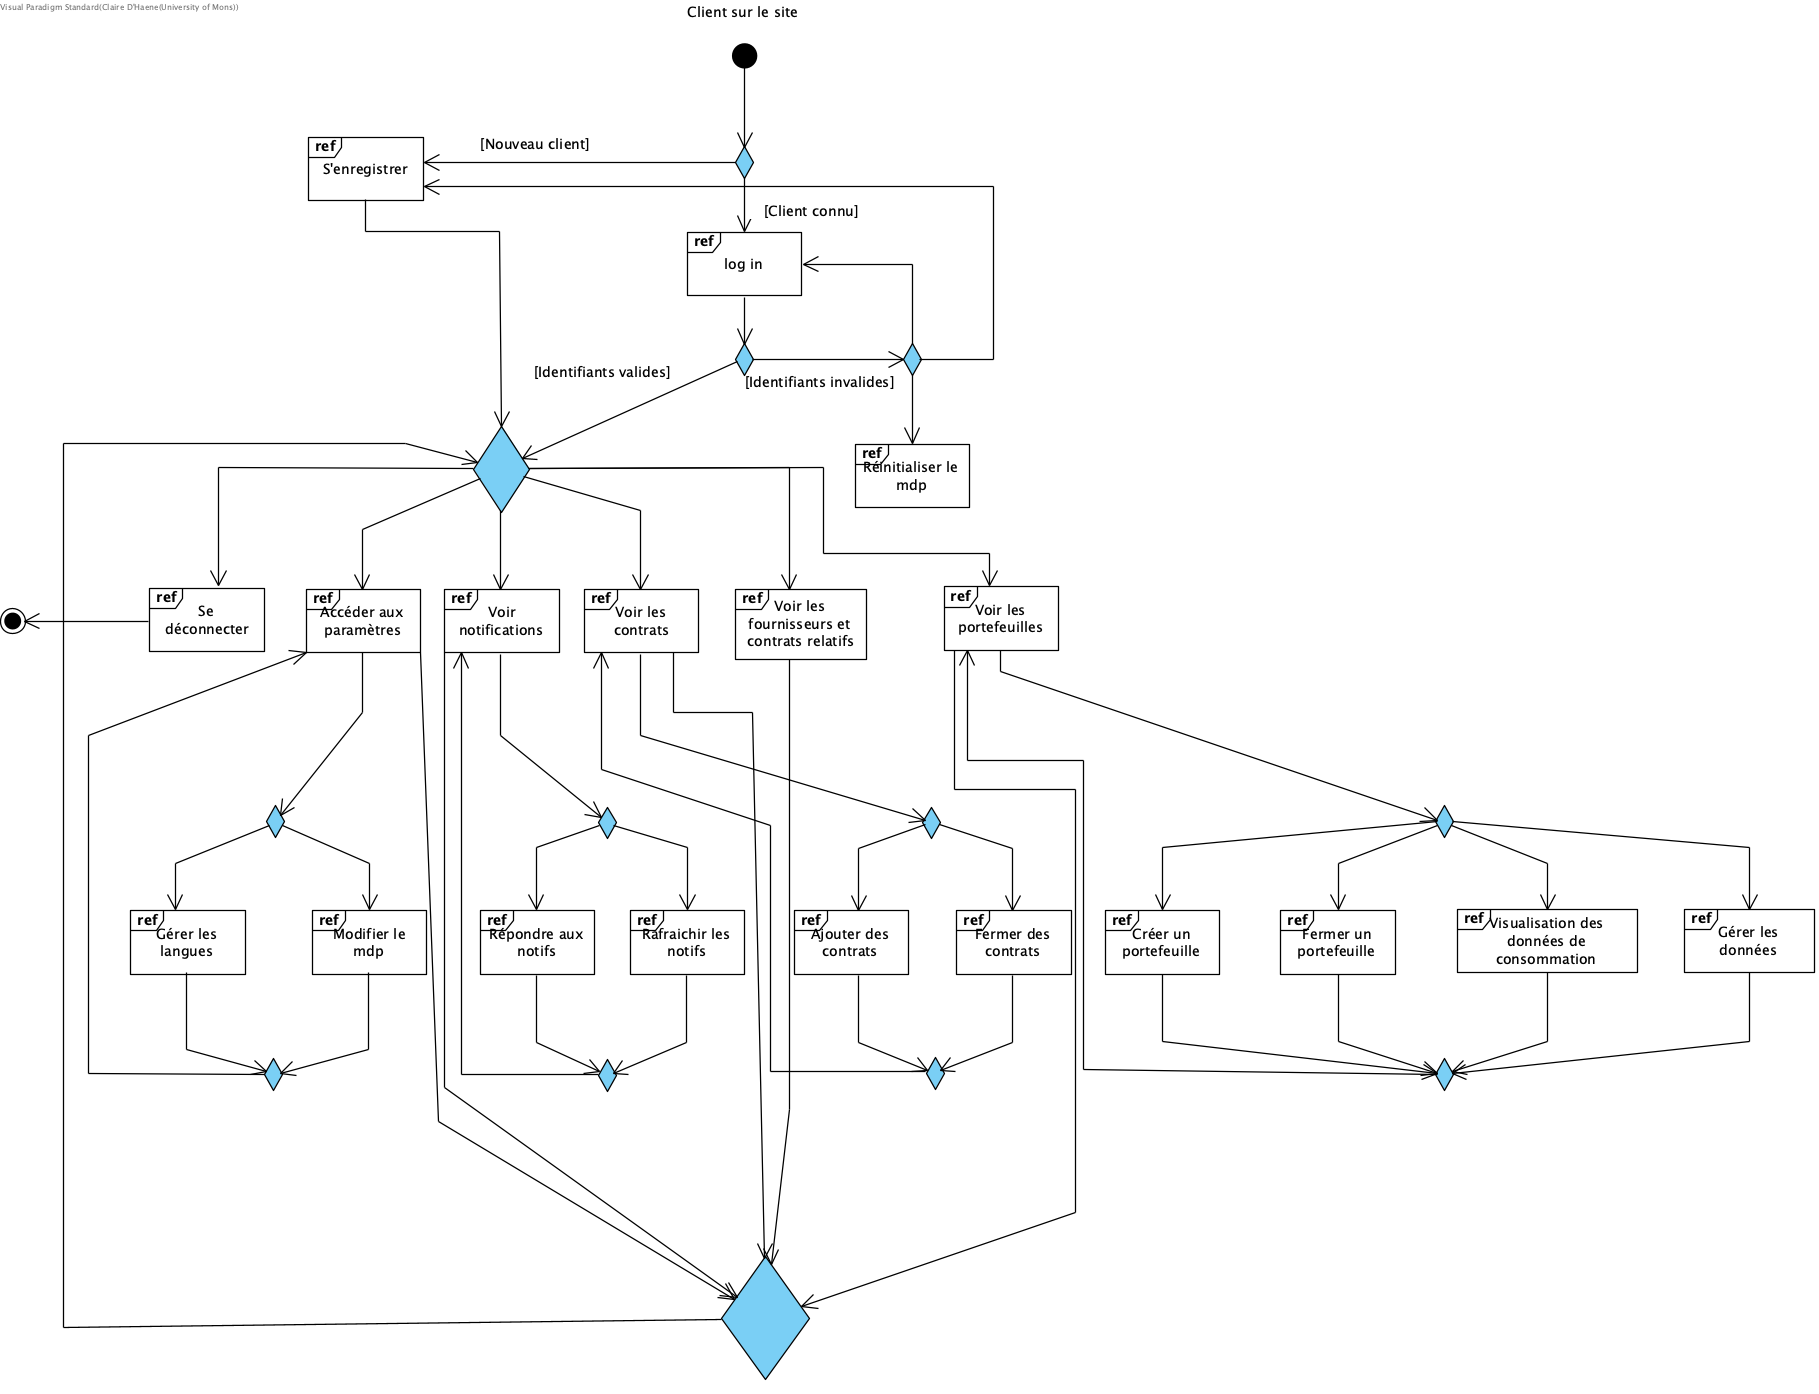
\includegraphics[width = 1\textwidth]{Base/interface/img/overview-client.png}
\end{figure}

\newpage
\subsection{Interface fournisseur}

Lorsqu'un fournisseur se connectera, il arrivera sur la page d'acceuil ou plus précisément "Home".
\begin{flushleft}
Ce dernier aura alors les possibilités suivantes :
\end{flushleft}
\begin{enumerate}
\item Voir ses clients ("Your clients")
\item Voir ses contrats ("Your contracts")
\item Voir ses notifications
\item Se déconnecter
\item Aller sur la page des paramètres
\end{enumerate}

\begin{flushleft}
Tout comme pour l'interface client, il est important de noter que ce n'est qu'à partir de ces six pages que le fournisseur pourra revenir sur la page "Home" étant donné le choix effectué dans notre overview diagram.
\end{flushleft}

\begin{flushleft}
Néanmoins, ce dernier aura la possibilité de revenir en arrière à l'aide du bouton "Back" lorsqu'il sera sur des "sous-pages" de ces six sections principales.
\end{flushleft}

\newpage

\begin{flushleft}
La première section est \textbf{Voir ses clients ("Your clients")}
\end{flushleft}

\begin{flushleft}
Le founisseur pourra à partir d'ici voir une liste reprenant tous les noms de ses clients ainsi que leurs adresses mails. 
\end{flushleft}

\begin{flushleft}
\textbf{Le bouton "Go"} lui permettra de voir plus en détail un client, il aura accès à :
\end{flushleft}
\begin{enumerate}
\item Son nom
\item Son adresse mail
\item Les contrats lui étant associés (Nom du contrat, code "EAN", le type d'énergie, la dernière consommation) : \newline
Le bouton "Go" lui donnera la possibilité de voir plus en détail le contrat de la même manière que lorsqu'un client souhaite voir ses contrats.\newline
Il aura la faculté de supprimer un contrat et voir les consommations.\newline
Contrairement au client, il ne pourra pas ajouter de nouvelles données de consommations mais simplement les modifier et les supprimer et ne pourra pas exporter les données mais en importer.
\item La suppresion d'un client (Bouton "Delete Client")
\end{enumerate}

\begin{flushleft}
Le \textbf{bouton "Add clients"} le mènera sur une page où il pourra sélectionner un contrat à envoyer à un possible nouveau client.
\end{flushleft}

\newpage

\begin{flushleft}
Passons à la deuxième section : \textbf{Voir ses contrats ("Your contracts")}
\end{flushleft}

\begin{flushleft}
Le founisseur pourra à partir d'ici voir une liste reprenant tous les noms de ses contrats, leurs types d'énergie ainsi que leurs localisations. 
\end{flushleft}

\begin{flushleft}
\textbf{Le bouton "Go"} lui donnera la possibilité de voir plus en détails ses contrats avec :
\end{flushleft}
\begin{enumerate}
\item Le nom du contrat
\item Le type d'énergie
\item La localisation (du contrat)
\item Le prix basique
\item Le prix dépendant du jour et la nuit
\item Le taux fixe ou variable
\item Les heures creuses
\item Le type de compteur
\end{enumerate}

\begin{flushleft}
Ce dernier aura également accès à la suppression du contrat et au changement du contrat fonctionnant comme \textbf{l'ajout de contrats (Bouton "Add contracts")} que nous allons expliquer ci-dessous.
\end{flushleft}

\begin{flushleft}
Lorsqu'un fournisseur souhaitera ajouter un contrat il devra entrer :
\end{flushleft}
\begin{enumerate}
\item Le nom du contrat
\item Le type d'énergie
\item La localisation (du contrat)
\item Le prix basique
\item Le prix dépendant du jour et la nuit
\item Les heures creuses
\item Le taux fixe ou variable
\item Le type de compteur
\end{enumerate}

\begin{flushleft}
Le bouton "Add" lui servira à valider la création du nouveau contrat.
\end{flushleft}

\begin{figure}
    \centering
    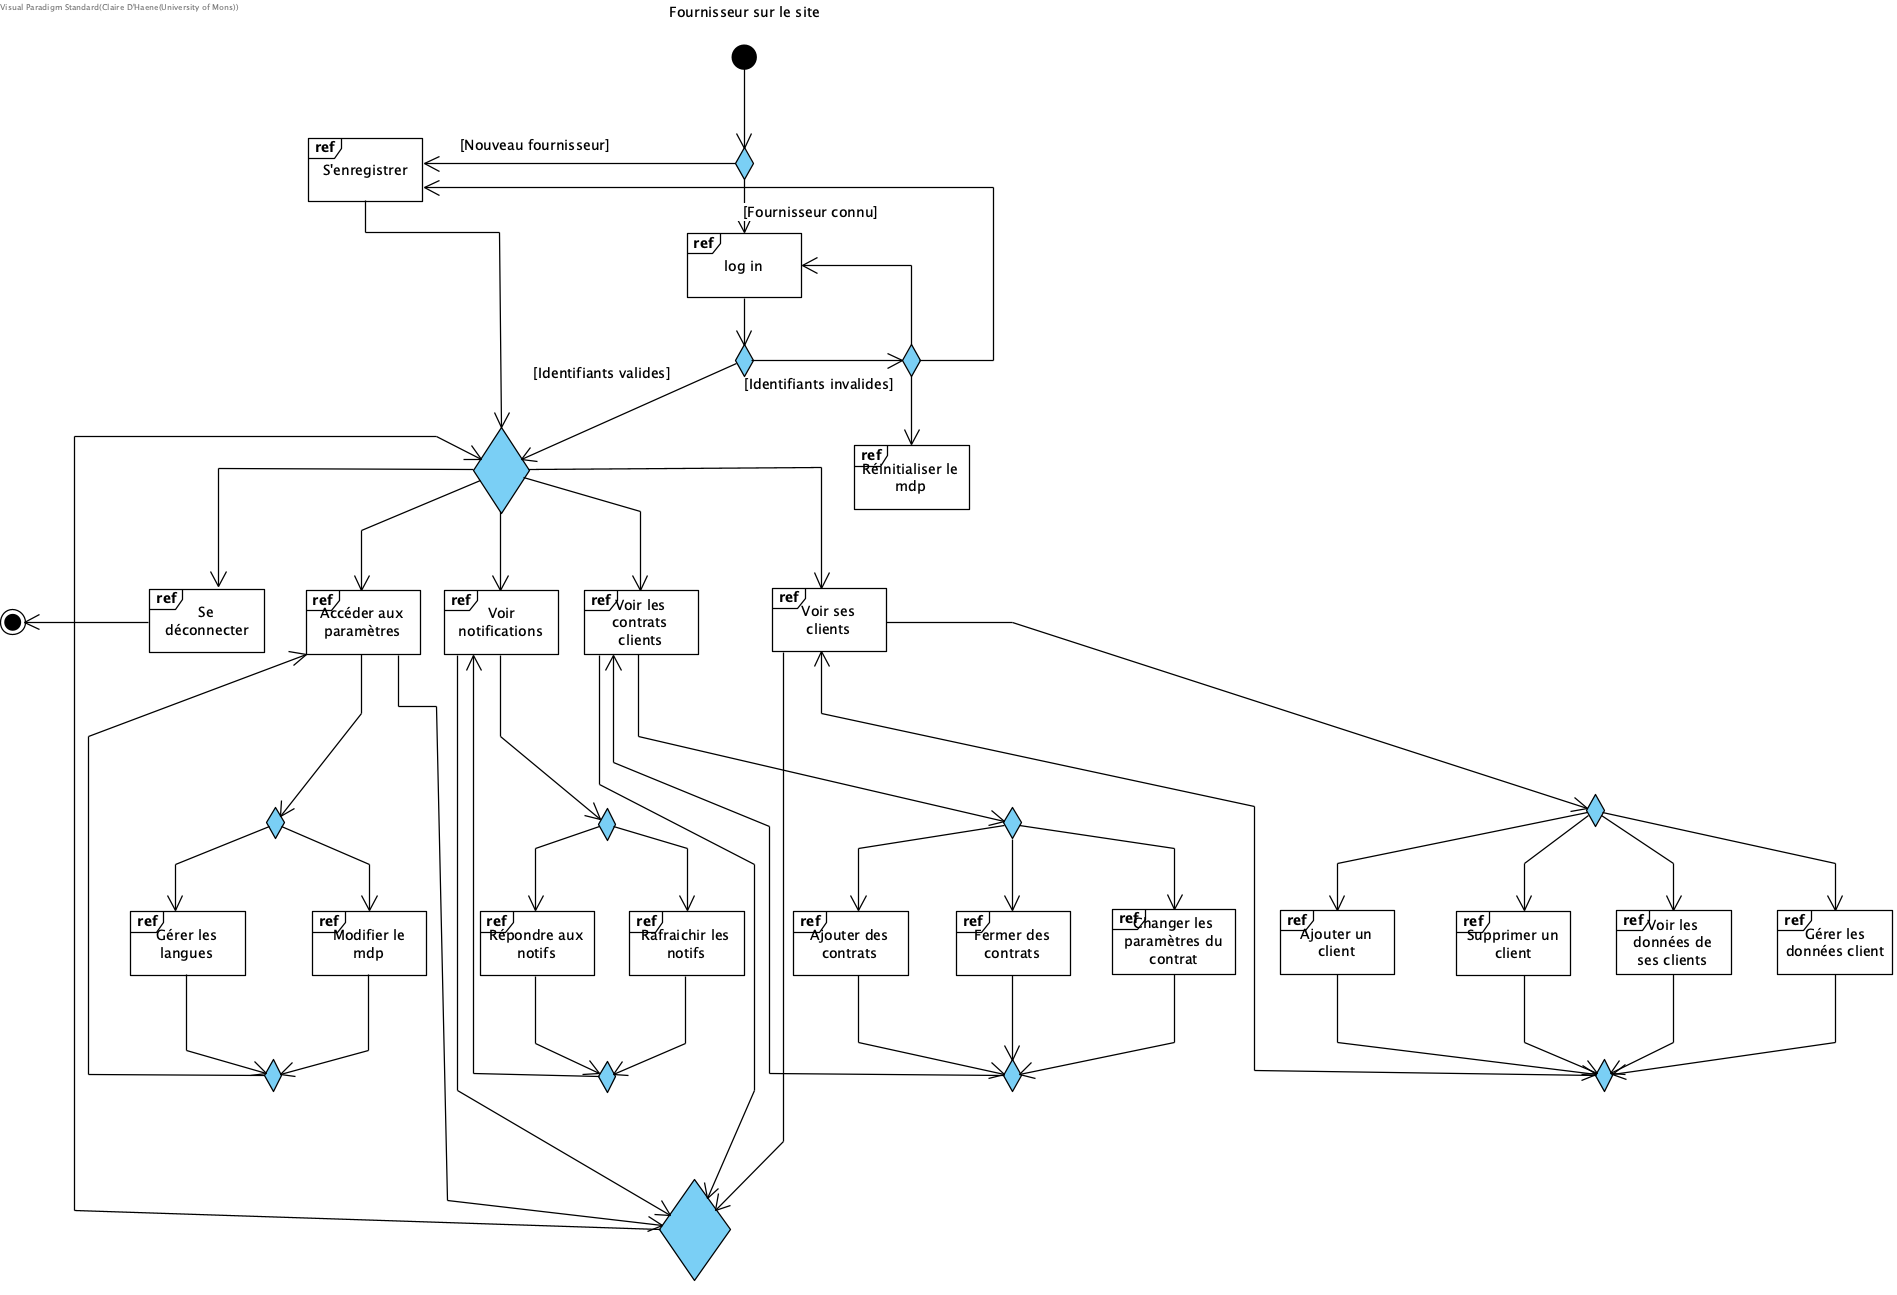
\includegraphics[width = 1\textwidth]{Base/interface/img/overview-fournisseur.png}
\end{figure}
